\begin{center}
    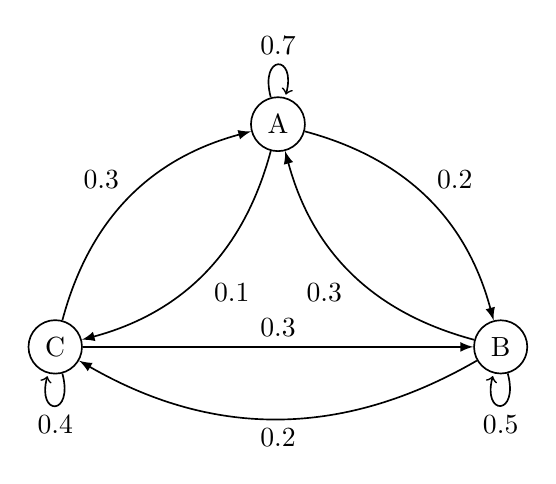
\begin{tikzpicture}[-latex, auto, node distance={4cm}, semithick, main/.style = {draw, circle}]
        \node[main] (A) {A};
        \node[main, below right of = A] (B) {B};
        \node[main, below left of = A] (C) {C}; 
        \path (A) edge[loop above] node{0.7} (A); 
        \path (A) edge[bend left] node{0.1} (C); 
        \path (A) edge[bend left] node{0.2} (B); 
        \path (B) edge[loop below] node{0.5} (B); 
        \path (B) edge[bend left] node{0.3} (A); 
        \path (B) edge[bend left] node{0.2} (C); 
        \path (C) edge node{0.3} (B); 
        \path (C) edge[bend left] node{0.3} (A); 
        \path (C) edge[loop below] node{0.4} (C); 
    \end{tikzpicture}
\end{center}
